\section{Development Environment}
\begin{frame}[fragile]
  \frametitle{Development Environment}
  \framesubtitle{\texttt{ipython notebook}}
  \begin{columns}[c]
    \column{1.0\textwidth}
      \lstset{tabsize=2,  language=Tex, basicstyle=\normalsize\ttfamily,
      breaklines=true, escapechar=*,  upquote=true}
      \begin{lstlisting}
$ ipython notebook --pylab='inline' 
                   --ip='0.0.0.0' 
                   --port=9999
\end{lstlisting}
    \end{columns}

    \vfill

    \begin{columns}[c]
    \column{1.0\textwidth}
      \begin{center}
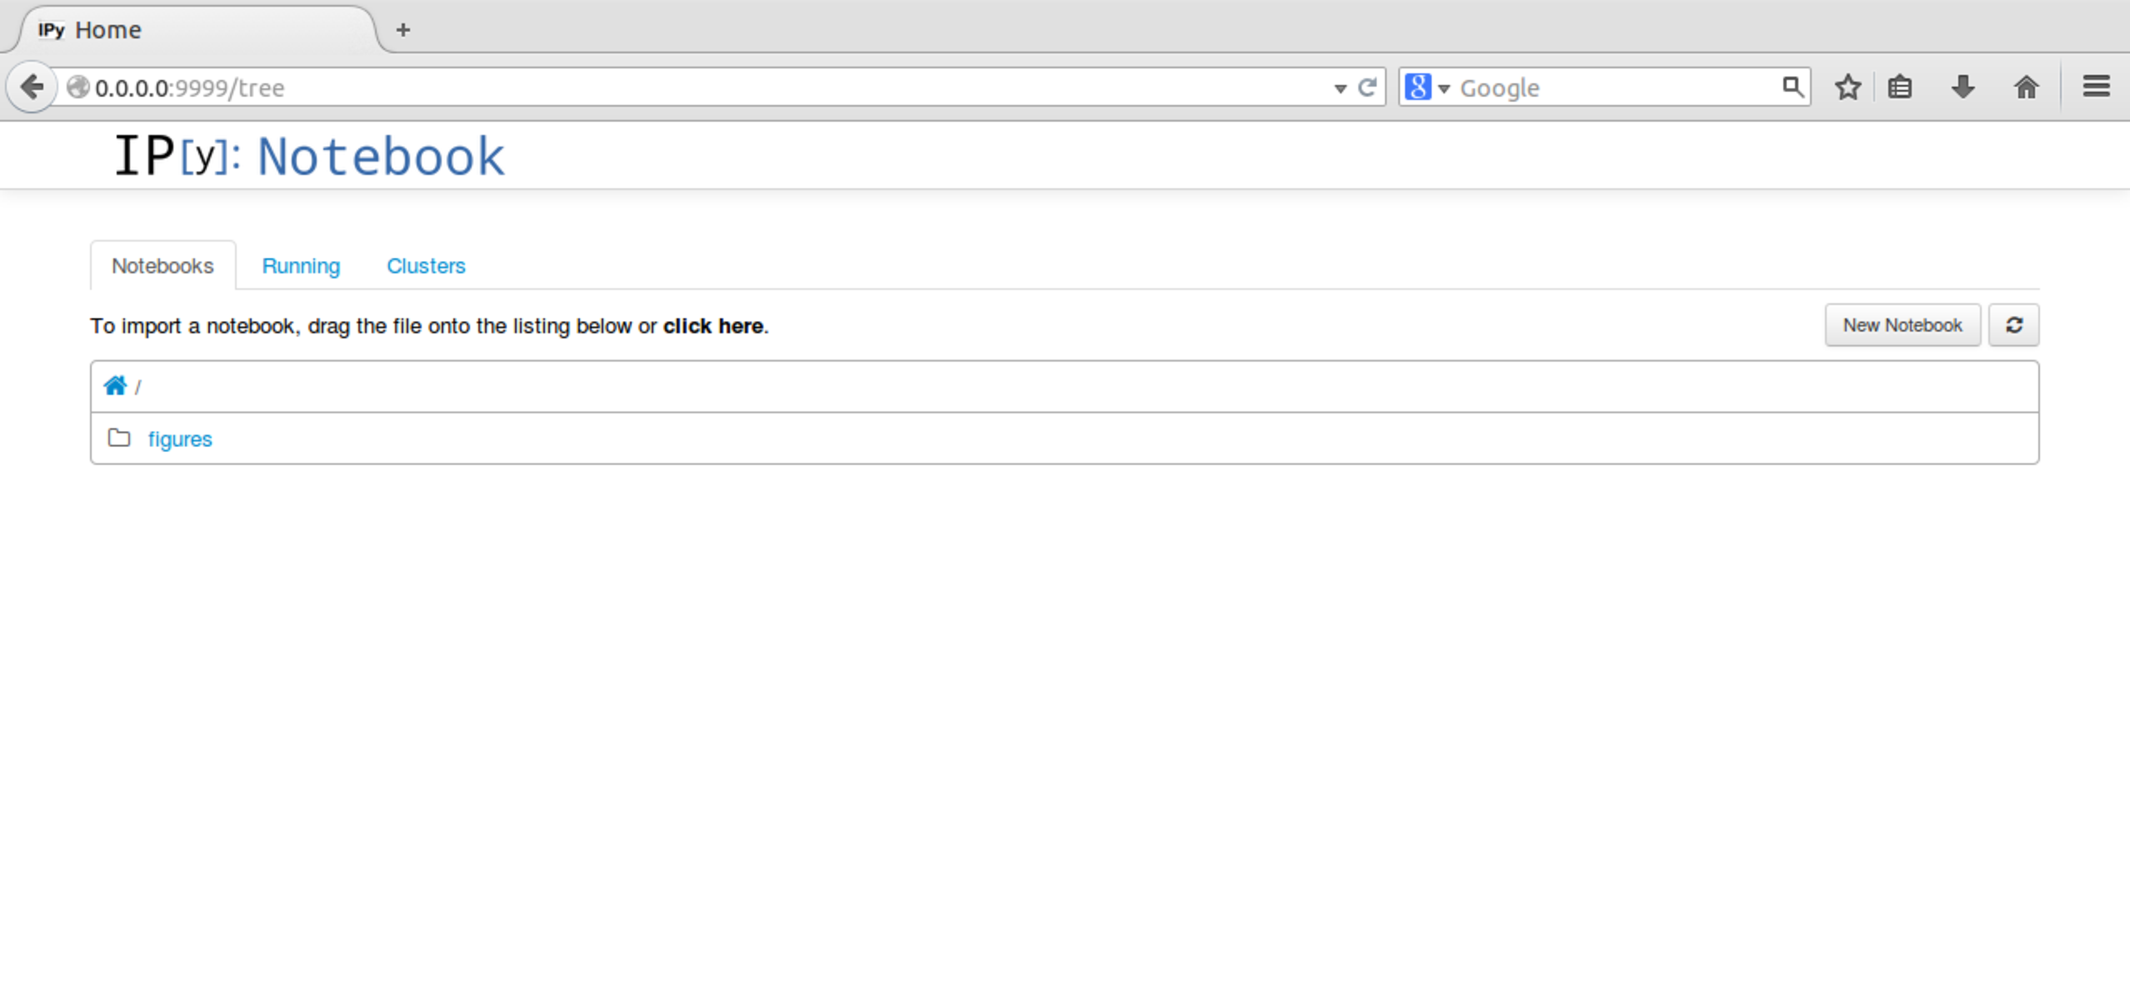
\includegraphics[width=1.0\linewidth]{figures/ipython-notebook-with-cmd}\\
    \end{center}
  \end{columns}
\end{frame}

